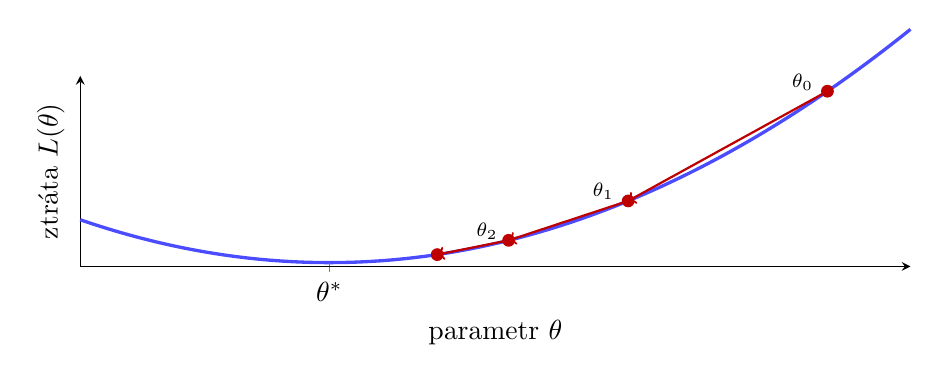
\begin{tikzpicture}
    \begin{axis}[
        width=\textwidth,
        height=4cm,
        xmin=0, xmax=5,
        ymin=0, ymax=10,
        axis lines=left,
        xlabel={parametr \(\theta\)},
        ylabel={ztráta \(L(\theta)\)},
        xtick={1.5},
        xticklabels={\(\theta^\ast\)},
        ytick=\empty,
        clip=false
    ]
        \addplot[
            very thick,
            blue!70,
            domain=0:5,
            samples=120
        ] {(x-1.5)^2+0.2};

        \addplot[
            only marks,
            mark=*,
            mark size=2.1pt,
            red!75!black
        ] coordinates {
            (4.5,9.2)
            (3.3,3.44)
            (2.58,1.37)
            (2.15,0.62)
        };

        \draw[->, thick, red!75!black]
            (axis cs:4.5,9.2) -- (axis cs:3.3,3.44);
        \draw[->, thick, red!75!black]
            (axis cs:3.3,3.44) -- (axis cs:2.58,1.37);
        \draw[->, thick, red!75!black]
            (axis cs:2.58,1.37) -- (axis cs:2.15,0.62);

        \node[font=\scriptsize] at (axis cs:4.35,9.65) {\(\theta_0\)};
        \node[font=\scriptsize] at (axis cs:3.15,3.95) {\(\theta_1\)};
        \node[font=\scriptsize] at (axis cs:2.45,1.85) {\(\theta_2\)};

        \addplot[
            dashed,
            gray
        ] coordinates {
            (1.5,0)
            (1.5,0.2)
        };
    \end{axis}
\end{tikzpicture}
